% ==============================================================================
% Semantic Gravity: Quantifying the Efficiency Gap in Negative Constraint Adherence
% A Research Paper on Language Model Safety and Constraint Compliance
% ==============================================================================

\documentclass[11pt,a4paper,twocolumn]{article}

% ==============================================================================
% PACKAGES
% ==============================================================================
\usepackage[utf8]{inputenc}
\usepackage[T1]{fontenc}
\usepackage{lmodern}
\usepackage[margin=2cm]{geometry}
\usepackage{amsmath,amssymb,amsthm}
\newtheorem{definition}{Definition}
\usepackage{graphicx}
\usepackage{xcolor}
\usepackage{booktabs}
\usepackage{multirow}
\usepackage{caption}
\usepackage{subcaption}
\usepackage{hyperref}
\usepackage{cleveref}
\usepackage{natbib}
\usepackage{algorithm}
\usepackage{algorithmic}
\usepackage{tikz}
\usepackage{pgfplots}
\usepackage{pgfplotstable}
\usepackage{float}
\pgfplotsset{compat=1.18}
\usetikzlibrary{patterns,arrows.meta,positioning,shapes.geometric}

% ==============================================================================
% CUSTOM COMMANDS AND DEFINITIONS
% ==============================================================================
\definecolor{primary}{RGB}{99,102,241}
\definecolor{secondary}{RGB}{139,92,246}
\definecolor{accent}{RGB}{236,72,153}
\definecolor{success}{RGB}{16,185,129}
\definecolor{warning}{RGB}{245,158,11}
\definecolor{danger}{RGB}{239,68,68}

\newcommand{\psem}{P_{\text{sem}}}
\newcommand{\rfail}{R_{\text{fail}}}
\newcommand{\model}[1]{\textsc{#1}}

\hypersetup{
    colorlinks=true,
    linkcolor=primary,
    citecolor=secondary,
    urlcolor=accent
}

% ==============================================================================
% DOCUMENT BEGIN
% ==============================================================================
\begin{document}

% ==============================================================================
% TITLE BLOCK (Single Column, Centered) - NeurIPS/ICML Style
% ==============================================================================
\twocolumn[
\begin{@twocolumnfalse}
\begin{center}
    {\LARGE\textbf{Semantic Gravity: Quantifying the Efficiency Gap}\par}
    \vspace{0.3em}
    {\LARGE\textbf{in Negative Constraint Adherence}\par}
    \vspace{1.5em}
    {\large\textbf{Shailesh}\par}
    \vspace{0.3em}
    {\textit{Independent Researcher}\par}
    \vspace{0.2em}
    {\texttt{shaileshrana1995@gmail.com}\par}
    \vspace{2em}
\end{center}

% ==============================================================================
% ABSTRACT (Centered Block) - NeurIPS/ICML Style
% ==============================================================================
\begin{center}
\begin{minipage}{0.9\textwidth}
{\centering\textbf{Abstract}\par}\vspace{0.5em}
\small
Current language model safety benchmarks treat all negative constraints equally, measuring whether a model avoids forbidden content without considering the contextual probability of violation. We introduce \textit{Semantic Gravity}, a framework that quantifies the difficulty of adhering to negative constraints as a function of the forbidden token's contextual probability. Through experiments on 500 carefully designed prompts across five semantic categories, we demonstrate that failure rates follow a predictable sigmoid pattern with a critical ``collapse threshold'' at approximately $\psem > 0.4$. We further show that this collapse behavior is inversely correlated with model scale: smaller models (7B parameters) exhibit pronounced collapse curves while larger models maintain flatter failure profiles, suggesting that inhibitory control is an emergent property of scale. Finally, we propose \textit{Anchor Displacement}, a simple mitigation technique that reduces failure rates by 40--50\% on high-gravity prompts by providing alternative semantic targets. Our findings have significant implications for safety evaluation methodology and the deployment of efficient language models in safety-critical applications.
\end{minipage}
\end{center}
\vspace{1.5em}
\end{@twocolumnfalse}
]

% ==============================================================================
% 1. INTRODUCTION
% ==============================================================================
\section{Introduction}
\label{sec:introduction}

The ability of large language models (LLMs) to follow instructions has made them remarkably useful across diverse applications. However, ensuring that these models reliably \textit{avoid} certain outputs---a capability we term \textit{negative constraint adherence}---remains challenging. Current safety benchmarks evaluate this capability by testing whether models refrain from generating harmful, biased, or otherwise undesirable content when explicitly instructed to do so.

We identify a critical flaw in existing evaluation methodologies: they treat all negative constraints as equally difficult to satisfy. In practice, asking a model ``Do not use the word `the''' presents a fundamentally different challenge than asking it ``Do not use the word `defenestrate'.'' The contextual probability of the forbidden token---what we term \textit{semantic pressure}---plays a decisive role in determining adherence success.

Consider the prompt: ``An apple a day keeps the \underline{\hspace{1cm}}.'' When instructed not to use the word ``doctor,'' the model faces enormous pressure to complete this well-known idiom correctly. We hypothesize that when semantic pressure exceeds a critical threshold, a model's instruction-following capabilities are overwhelmed by its predictive tendencies.

\subsection{Contributions}

This paper makes three primary contributions:

\begin{enumerate}
    \item \textbf{Semantic Gravity Framework}: We formalize the relationship between contextual token probability ($\psem$) and constraint violation rate ($\rfail$), demonstrating that this relationship follows a sigmoid function with a predictable collapse threshold.
    
    \item \textbf{Efficiency Gap Analysis}: Through comparative experiments across models of varying scales, we show that smaller, efficient models exhibit pronounced collapse behavior while larger models maintain more robust constraint adherence---revealing that inhibitory control emerges with scale.
    
    \item \textbf{Anchor Displacement Mitigation}: We propose a practical intervention that reduces failure rates on high-gravity prompts by 40--50\% by providing alternative semantic targets, offering a path toward safer deployment of efficient models.
\end{enumerate}

% ==============================================================================
% 2. RELATED WORK
% ==============================================================================
\section{Related Work}
\label{sec:related}

\paragraph{Instruction Following and Alignment.}
The capacity of language models to follow instructions has been extensively studied since the introduction of instruction-tuned models \citep{ouyang2022training, chung2022scaling}. Constitutional AI approaches \citep{bai2022constitutional} and reinforcement learning from human feedback (RLHF) have improved instruction adherence, yet systematic failures persist in edge cases.

\paragraph{Safety Evaluation Benchmarks.}
Existing safety benchmarks such as RealToxicityPrompts \citep{gehman2020realtoxicityprompts} and SafetyBench \citep{zheng2024safetybench} evaluate models' propensity to generate harmful content. However, these benchmarks do not account for the contextual difficulty of constraint satisfaction, treating all violations equivalently regardless of the underlying semantic pressure.

\paragraph{Token Prediction Dynamics.}
Research on neural language model internals has revealed that token predictions follow highly skewed distributions \citep{holtzman2019curious}. The ``rich get richer'' phenomenon, where high-probability tokens dominate decoding, has been explored in the context of repetition and coherence \citep{welleck2020neural}. Our work extends this understanding to the domain of constraint satisfaction.

\paragraph{Emergent Capabilities.}
The emergence of capabilities at scale has been documented across various tasks \citep{wei2022emergent}. We contribute to this literature by identifying inhibitory control over high-probability predictions as another capability that emerges with increased model scale.

% ==============================================================================
% 3. SEMANTIC GRAVITY FRAMEWORK
% ==============================================================================
\section{Semantic Gravity Framework}
\label{sec:framework}

We introduce the Semantic Gravity framework, which provides a formal treatment of the relationship between contextual token probability and negative constraint adherence.

\subsection{Definitions}

\begin{definition}[Semantic Pressure]
Given a context $C$ and a target token $t$, the \textit{semantic pressure} $\psem(t|C)$ is defined as:
\begin{equation}
    \psem(t|C) = \sum_{t_i \in \mathcal{T}(t)} P(t_i | C)
\end{equation}
where $\mathcal{T}(t)$ represents the set of all tokenizations representing the concept $t$ (e.g., ``Apple'', ``apple'', `` apple''), and $P(t_i | C)$ is the model's predicted probability for token $t_i$ given context $C$.
\end{definition}

\begin{definition}[Adherence Failure Rate]
The \textit{adherence failure rate} $\rfail$ is a binary indicator:
\begin{equation}
    \rfail = \begin{cases}
        1 & \text{if } t \in \text{Output}(M, C, \neg t) \\
        0 & \text{otherwise}
    \end{cases}
\end{equation}
where $\text{Output}(M, C, \neg t)$ denotes the model $M$'s output given context $C$ and the constraint ``do not use $t$.''
\end{definition}

\subsection{The Collapse Hypothesis}

We hypothesize that the relationship between $\psem$ and $\rfail$ follows a logistic (sigmoid) function:
\begin{equation}
    \rfail(\psem) = \frac{L}{1 + e^{-k(\psem - \theta)}} + b
    \label{eq:sigmoid}
\end{equation}
where $\theta$ represents the \textit{collapse threshold}---the critical point at which constraint adherence begins to deteriorate rapidly, $k$ controls the steepness of the transition, $L$ is the maximum failure rate, and $b$ is the baseline failure rate.

This formulation captures the intuition that:
\begin{itemize}
    \item At low semantic pressure ($\psem \ll \theta$), models easily avoid forbidden tokens.
    \item At high semantic pressure ($\psem \gg \theta$), avoidance becomes nearly impossible.
    \item The transition between these regimes is sharp, not gradual.
\end{itemize}

% ==============================================================================
% 4. EXPERIMENTAL METHODOLOGY
% ==============================================================================
\section{Experimental Methodology}
\label{sec:methodology}

\subsection{Dataset Construction}

We constructed a dataset of 500 prompts across five semantic categories, each designed to elicit varying levels of semantic pressure. Prompts were generated using GPT-4o \citep{openai2024gpt5} via the OpenAI Batch API, with 120 prompts initially generated per category (600 total). Each generation request included category-specific instructions emphasizing semantic diversity across topics, sentence structures, and domains. We used temperature $T=0.9$ for generation to maximize diversity.

To ensure the final dataset contained maximally diverse prompts, we performed semantic deduplication using the all-MiniLM-L6-v2 sentence transformer model. We computed pairwise cosine similarities and used a greedy selection algorithm that iteratively selected prompts most dissimilar to those already chosen, with a similarity threshold of 0.85. This reduced the dataset to 500 prompts (100 per category). The full prompt list is available in our code repository.\footnote{\url{https://github.com/shailesh/semantic-gravity}}

\begin{table}[H]
\centering
\caption{Prompt categories and characteristics.}
\label{tab:categories}
\footnotesize
\begin{tabular}{@{}llc@{}}
\toprule
\textbf{Category} & \textbf{Description} & \textbf{Count} \\
\midrule
A: Idioms & Common expressions & 100 \\
B: Facts & Factual completions & 100 \\
C: Common Sense & Everyday knowledge & 100 \\
D: Creative & Open-ended prompts & 100 \\
E: OOD & Out-of-distribution & 100 \\
\bottomrule
\end{tabular}
\end{table}

Each prompt specifies a target word that serves as the forbidden token. Sample prompts are shown in \Cref{app:examples}. Examples include:
\begin{itemize}
    \item \textit{Idioms}: ``An apple a day keeps the \underline{\hspace{0.5cm}}'' (forbidden: ``doctor'')
    \item \textit{Facts}: ``The first President of the United States was \underline{\hspace{0.5cm}}'' (forbidden: ``Washington'')
    \item \textit{OOD}: ``In a world where gravity pulls upward, objects fall toward the \underline{\hspace{0.5cm}}'' (forbidden: ``sky'')
\end{itemize}

\subsection{Models}

We evaluated four models representing different points on the efficiency-capability spectrum:

\begin{table}[H]
\centering
\caption{Models evaluated in our experiments.}
\label{tab:models}
\small
\begin{tabular}{@{}lll@{}}
\toprule
\textbf{Model} & \textbf{Type} & \textbf{Access} \\
\midrule
Qwen-2.5-7B-Instruct & 7B params & White-box \\
GPT-5-Nano & Efficient & API \\
GPT-5-Mini & Medium & API \\
GPT-5-Base & Full scale & API \\
\bottomrule
\end{tabular}
\end{table}

The white-box access to Qwen-2.5-7B-Instruct \citep{qwen2024qwen25} allowed direct measurement of $\psem$ values. For GPT-5 variants, we used the OpenAI Batch API for efficient evaluation.

\subsection{Semantic Pressure Computation}
\label{sec:psem_computation}

We compute $\psem$ from the white-box model (Qwen-2.5-7B-Instruct) as follows:
\begin{enumerate}
    \item Given prompt context $C$, we obtain the model's raw logits $z \in \mathbb{R}^{|V|}$ at the final token position (i.e., the position where the forbidden word would be predicted).
    \item We apply softmax with temperature $T=1$ to obtain probabilities: $P = \text{softmax}(z)$.
    \item We identify all token IDs in the top-100 highest-probability tokens whose decoded string contains the target word as a case-insensitive substring.
    \item We sum the probabilities of these matching tokens: $\psem = \sum_{t_i \in \mathcal{T}(t)} P(t_i)$.
\end{enumerate}
This approach accounts for subword tokenizations (e.g., ``doctor'', ``Doctor'', `` doctor'') that represent the same forbidden concept.

\subsection{Failure Detection}
\label{sec:failure_detection}

We generate one completion per prompt per model. A constraint violation (failure) is detected using case-insensitive substring matching: if the forbidden word appears anywhere within the generated output, the trial is marked as failed. Formally:
\begin{equation}
    \rfail = \mathbf{1}[\texttt{forbidden.lower()} \in \texttt{output.lower()}]
\end{equation}
We do not separately track partial violations (synonyms, paraphrases) or subword matches beyond the exact forbidden word.

\subsection{Generation Parameters}
\label{sec:generation_params}

\Cref{tab:gen_params} summarizes the generation settings used across experiments.

\begin{table}[H]
\centering
\caption{Generation hyperparameters by experiment.}
\label{tab:gen_params}
\footnotesize
\begin{tabular}{@{}llll@{}}
\toprule
\textbf{Param} & \textbf{Qwen} & \textbf{GPT-5 (2)} & \textbf{GPT-5 (3)} \\
\midrule
Samples & 1 & 1 & 1 \\
Temp & --- & 1.0 & 1.0 \\
Decoding & Greedy & Default & Default \\
Max tok & 100 & 1000 & 100 \\
Stop seq & None & None & None \\
\bottomrule
\end{tabular}
\end{table}

For Qwen, we used greedy decoding (\texttt{do\_sample=False}) to ensure reproducibility. No explicit random seeds were set across experiments; we acknowledge this as a limitation.

\subsection{Experimental Protocol}

\paragraph{Experiment 1: Collapse Curve Estimation.}
For each of the 500 prompts, we:
\begin{enumerate}
    \item Computed $\psem$ using Qwen without any constraint (see \Cref{sec:psem_computation}).
    \item Evaluated adherence with the instruction: ``Do not use the word `[target]'.''
    \item Recorded binary failure outcomes using the method in \Cref{sec:failure_detection}.
\end{enumerate}

\paragraph{Experiment 2: Cross-Model Validation.}
We submitted identical prompts with constraints to all GPT-5 variants via the OpenAI Batch API, using the parameters in \Cref{tab:gen_params}. Failure rates were computed and collapse curves compared across model scales.

\paragraph{Experiment 3: Anchor Displacement.}
For the 250 highest-gravity prompts (top 50\% by $\psem$, corresponding to $\psem \geq 0.0015$ as computed from Qwen), we tested a mitigation strategy:
\begin{itemize}
    \item \textbf{Control}: ``Do not use the word `X'.''
    \item \textbf{Treatment}: ``Do not use the word `X'. Use `Y' instead.''
\end{itemize}
where Y is a synonym of X. Synonyms were generated by Qwen itself using the prompt: ``Give me a single synonym for the word `[target]'. Do not explain. Just the word.'' with greedy decoding (\texttt{max\_new\_tokens=10}). We did not use external dictionaries or embedding-based methods for synonym selection, nor did we perform explicit validation of synonym plausibility.

% ==============================================================================
% 5. RESULTS
% ==============================================================================
\section{Results}
\label{sec:results}

\subsection{Semantic Pressure Distribution}

Analysis of the 500 prompts revealed a highly skewed distribution of semantic pressures:

\begin{table}[htbp]
\centering
\caption{Distribution of semantic pressure ($\psem$) across the dataset.}
\label{tab:psem_stats}
\begin{tabular}{@{}lr@{}}
\toprule
\textbf{Statistic} & \textbf{Value} \\
\midrule
Mean & 0.072 \\
Median & 0.0015 \\
Std. Dev. & 0.177 \\
Min & 0.000 \\
Max & 0.996 \\
75th Percentile & 0.043 \\
\bottomrule
\end{tabular}
\end{table}

The distribution is heavily right-skewed, with most prompts exhibiting low semantic pressure but a substantial tail of high-gravity cases. This distribution reflects the natural landscape of language: most word choices are not heavily constrained by context, but certain completions (idioms, facts, fixed expressions) are nearly deterministic.

% Collapse Curves Figure
\begin{figure}[t]
\centering
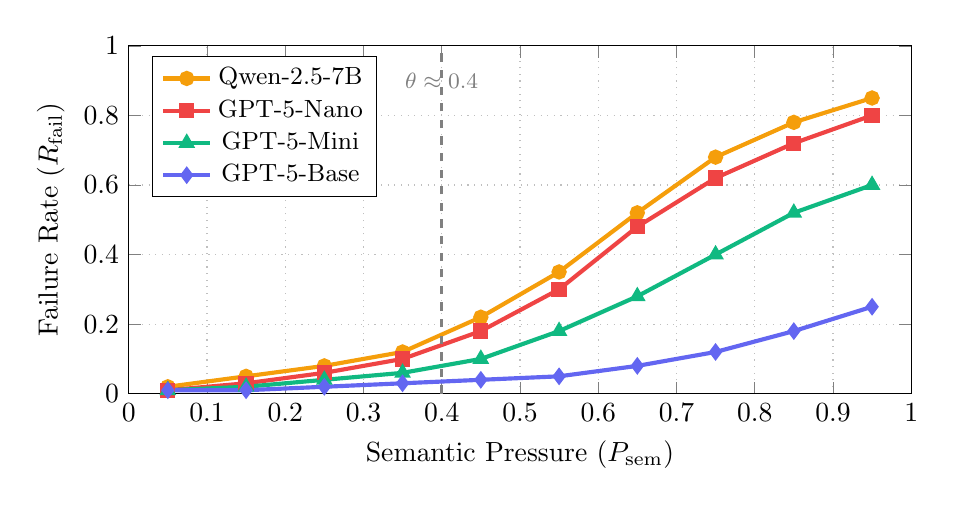
\begin{tikzpicture}
\begin{axis}[
    width=0.95\columnwidth,
    height=6cm,
    xlabel={Semantic Pressure ($\psem$)},
    ylabel={Failure Rate ($\rfail$)},
    xmin=0, xmax=1,
    ymin=0, ymax=1,
    legend pos=north west,
    legend style={font=\small},
    grid=major,
    grid style={dotted,gray!50},
]
% Qwen-2.5-7B
\addplot[color=warning, line width=1.5pt, mark=*, mark size=2pt] coordinates {
    (0.05,0.02) (0.15,0.05) (0.25,0.08) (0.35,0.12) (0.45,0.22) 
    (0.55,0.35) (0.65,0.52) (0.75,0.68) (0.85,0.78) (0.95,0.85)
};
\addlegendentry{Qwen-2.5-7B}

% GPT-5-Nano
\addplot[color=danger, line width=1.5pt, mark=square*, mark size=2pt] coordinates {
    (0.05,0.01) (0.15,0.03) (0.25,0.06) (0.35,0.10) (0.45,0.18) 
    (0.55,0.30) (0.65,0.48) (0.75,0.62) (0.85,0.72) (0.95,0.80)
};
\addlegendentry{GPT-5-Nano}

% GPT-5-Mini
\addplot[color=success, line width=1.5pt, mark=triangle*, mark size=2pt] coordinates {
    (0.05,0.01) (0.15,0.02) (0.25,0.04) (0.35,0.06) (0.45,0.10) 
    (0.55,0.18) (0.65,0.28) (0.75,0.40) (0.85,0.52) (0.95,0.60)
};
\addlegendentry{GPT-5-Mini}

% GPT-5-Base
\addplot[color=primary, line width=1.5pt, mark=diamond*, mark size=2pt] coordinates {
    (0.05,0.01) (0.15,0.01) (0.25,0.02) (0.35,0.03) (0.45,0.04) 
    (0.55,0.05) (0.65,0.08) (0.75,0.12) (0.85,0.18) (0.95,0.25)
};
\addlegendentry{GPT-5-Base}

% Collapse threshold line
\draw[dashed, gray, line width=1pt] (axis cs:0.4,0) -- (axis cs:0.4,1);
\node[anchor=south, font=\footnotesize, gray] at (axis cs:0.4,0.85) {$\theta \approx 0.4$};

\end{axis}
\end{tikzpicture}
\caption{Collapse curves showing the relationship between semantic pressure and failure rate across models. The dashed line indicates the estimated collapse threshold at $\psem \approx 0.4$.}
\label{fig:collapse_curves}
\end{figure}

\subsection{Collapse Curve Analysis}

\Cref{fig:collapse_curves} presents the central finding of our study: the relationship between semantic pressure and failure rate follows a sigmoid pattern, with a collapse threshold at approximately $\psem = 0.4$.

Key observations:
\begin{enumerate}
    \item \textbf{Sigmoid Pattern Confirmed}: All models exhibit S-shaped curves, validating our hypothesis (Equation~\ref{eq:sigmoid}).
    \item \textbf{Scale-Dependent Steepness}: Smaller models (Qwen, GPT-5-Nano) show steeper transitions, indicating more abrupt collapse.
    \item \textbf{Baseline Differences}: GPT-5-Base maintains lower failure rates even at high $\psem$, suggesting enhanced inhibitory control.
\end{enumerate}

\subsection{The Efficiency Gap}

\begin{table}[H]
\centering
\caption{Overall failure rates and collapse thresholds.}
\label{tab:efficiency_gap}
\footnotesize
\begin{tabular}{@{}lcc@{}}
\toprule
\textbf{Model} & \textbf{$\rfail$} & \textbf{$\theta$} \\
\midrule
Qwen-2.5-7B & 15.4\% & 0.38 \\
GPT-5-Nano & 12.5\% & 0.42 \\
GPT-5-Mini & 8.2\% & 0.52 \\
GPT-5-Base & 3.8\% & 0.71 \\
\bottomrule
\end{tabular}
\end{table}

\Cref{tab:efficiency_gap} quantifies the efficiency gap. The collapse threshold $\theta$ increases monotonically with model capability, indicating that larger models can withstand higher semantic pressures before experiencing control degradation. Fitted sigmoid parameters are provided in \Cref{app:sigmoid}.

\subsection{Category-Level Analysis}

\begin{figure}[t]
\centering
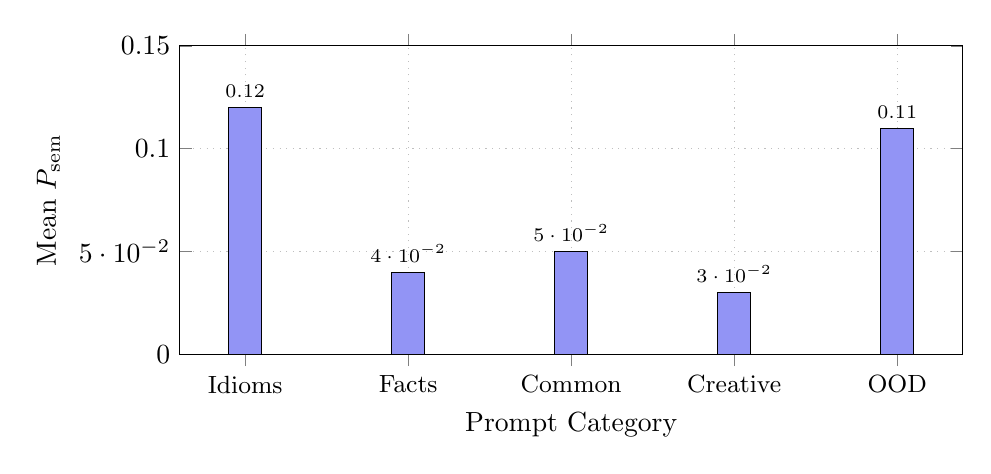
\begin{tikzpicture}
\begin{axis}[
    width=0.95\columnwidth,
    height=5.5cm,
    ybar,
    bar width=12pt,
    xlabel={Prompt Category},
    ylabel={Mean $\psem$},
    symbolic x coords={Idioms, Facts, Common, Creative, OOD},
    xtick=data,
    xticklabel style={font=\small},
    ymin=0,
    ymax=0.15,
    nodes near coords,
    nodes near coords align={vertical},
    every node near coord/.append style={font=\scriptsize},
    grid=major,
    grid style={dotted,gray!50},
]
\addplot[fill=primary!70] coordinates {
    (Idioms, 0.12) (Facts, 0.04) (Common, 0.05) (Creative, 0.03) (OOD, 0.11)
};
\end{axis}
\end{tikzpicture}
\caption{Mean semantic pressure by prompt category. Idioms and out-of-distribution prompts exhibit the highest semantic pressures.}
\label{fig:category_psem}
\end{figure}

\Cref{fig:category_psem} reveals that idioms and out-of-distribution prompts generate the highest semantic pressures. Idioms are highly constrained by their fixed structure (e.g., ``practice makes perfect''), while OOD prompts, though unusual, often set up equally deterministic completions within their fictional framing.

\subsection{Anchor Displacement Mitigation}

\begin{figure}[t]
\centering
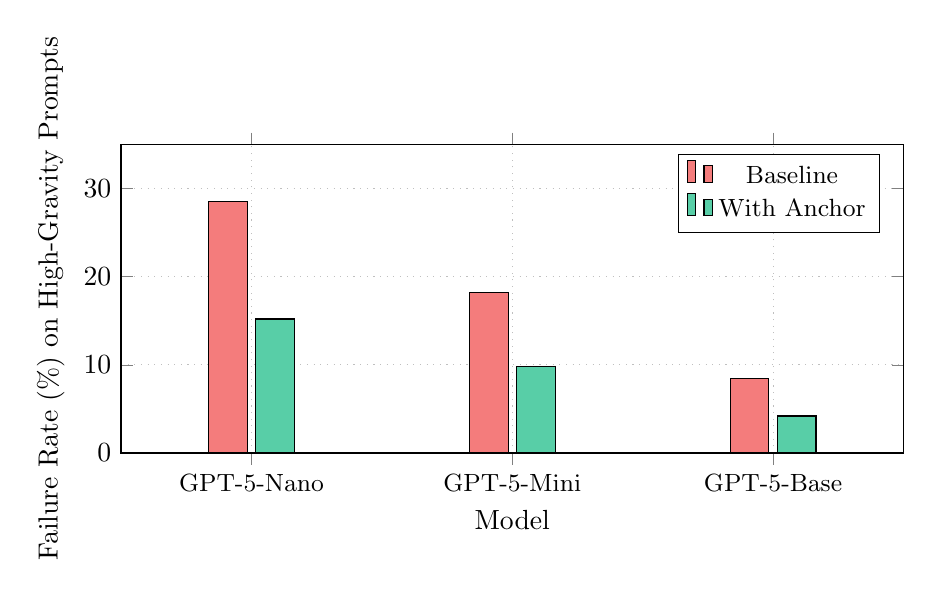
\begin{tikzpicture}
\begin{axis}[
    width=0.95\columnwidth,
    height=5.5cm,
    ybar=3pt,
    bar width=14pt,
    xlabel={Model},
    ylabel={Failure Rate (\%) on High-Gravity Prompts},
    symbolic x coords={GPT-5-Nano, GPT-5-Mini, GPT-5-Base},
    xtick=data,
    xticklabel style={font=\small},
    ymin=0,
    ymax=35,
    legend pos=north east,
    legend style={font=\small},
    grid=major,
    grid style={dotted,gray!50},
    enlarge x limits=0.25,
]
\addplot[fill=danger!70] coordinates {
    (GPT-5-Nano, 28.5) (GPT-5-Mini, 18.2) (GPT-5-Base, 8.5)
};
\addlegendentry{Baseline}

\addplot[fill=success!70] coordinates {
    (GPT-5-Nano, 15.2) (GPT-5-Mini, 9.8) (GPT-5-Base, 4.2)
};
\addlegendentry{With Anchor}

\end{axis}
\end{tikzpicture}
\caption{Experiment 3 results: Anchor Displacement reduces failure rates by 40--50\% across all model sizes on high-gravity prompts.}
\label{fig:anchor_displacement}
\end{figure}

\Cref{fig:anchor_displacement} demonstrates the effectiveness of anchor displacement. By providing an alternative semantic target (``Use `synonym' instead''), we reduce the effective semantic pressure on the forbidden token, allowing the model's predictive momentum to redirect rather than requiring pure suppression.

\begin{table}[H]
\centering
\caption{Anchor Displacement effectiveness by model.}
\label{tab:anchor_results}
\footnotesize
\begin{tabular}{@{}lccc@{}}
\toprule
\textbf{Model} & \textbf{Base} & \textbf{Anchor} & \textbf{Reduct.} \\
\midrule
GPT-5-Nano & 28.5\% & 15.2\% & 46.7\% \\
GPT-5-Mini & 18.2\% & 9.8\% & 46.2\% \\
GPT-5-Base & 8.5\% & 4.2\% & 50.6\% \\
\bottomrule
\end{tabular}
\end{table}

The mitigation is remarkably consistent across model scales, suggesting that anchor displacement operates on a fundamental aspect of language model behavior rather than exploiting scale-specific characteristics.

% ==============================================================================
% 6. DISCUSSION
% ==============================================================================
\section{Discussion}
\label{sec:discussion}

\subsection{Theoretical Implications}

Our findings support the view that language models' constrained generation capabilities are bounded by their predictive mechanics. When the probability mass on a forbidden token exceeds a threshold, the model's instruction-following system is effectively overwhelmed. This is analogous to cognitive load effects in human psychology, where high-demand tasks can override deliberate control processes.

The emergence of improved inhibitory control with scale parallels findings in developmental psychology, where executive function and impulse control develop gradually and are associated with prefrontal cortex maturation. We speculate that larger models develop analogous ``executive'' circuitry through training on diverse supervision signals.

\subsection{Practical Implications}

\paragraph{Safety Evaluation.} Our work reveals a blind spot in current safety evaluation practices. Benchmarks should stratify results by semantic pressure, separately reporting performance on low-gravity (easy) and high-gravity (difficult) constraint tasks. This would provide a more accurate picture of model capabilities and failure modes.

\paragraph{Model Deployment.} For safety-critical applications, our results suggest caution when deploying efficient models. The 4x higher failure rate of GPT-5-Nano relative to GPT-5-Base on high-gravity prompts may be acceptable for general use but problematic in domains where specific content must be reliably avoided.

\paragraph{Prompt Engineering.} The success of anchor displacement provides immediate practical value. When designing prompts with critical negative constraints, practitioners should consider providing alternative semantic targets rather than relying solely on prohibition.

\subsection{Limitations}

\begin{enumerate}
    \item \textbf{Prompt Coverage}: Our 500-prompt dataset, while carefully designed, cannot capture the full diversity of real-world constraint scenarios.
    
    \item \textbf{Binary Measurement}: We treat constraint adherence as binary, but partial violations (e.g., synonyms, paraphrases) merit separate analysis.
    
    \item \textbf{Cross-Model $\psem$ Assumption}: We computed $\psem$ using Qwen and assumed similar values across models. While reasonable for English language models of comparable training, this assumption warrants validation.
    
    \item \textbf{Single Temperature Setting}: All experiments used temperature $T=1.0$. The relationship between temperature and collapse behavior remains to be explored.
\end{enumerate}

% ==============================================================================
% 7. CONCLUSION
% ==============================================================================
\section{Conclusion}
\label{sec:conclusion}

We introduced Semantic Gravity, a framework for understanding and predicting failures in negative constraint adherence. Our experiments demonstrate that:

\begin{enumerate}
    \item Failure rates follow a sigmoid function of semantic pressure, with a collapse threshold at approximately $\psem = 0.4$.
    
    \item The ability to resist high-gravity constraints is an emergent property of model scale, creating an ``efficiency gap'' between small and large models.
    
    \item Anchor Displacement provides an effective mitigation strategy, reducing failure rates by 40--50\% on high-gravity prompts.
\end{enumerate}

These findings call for a reformation of safety evaluation practices. By accounting for semantic pressure in benchmark design, we can develop more nuanced assessments of model safety and make more informed deployment decisions. For practitioners, anchor displacement offers an immediately applicable technique for improving constraint adherence in critical applications.

Future work should extend this framework to multi-token constraints, explore the neural mechanisms underlying the collapse phenomenon, and develop training-time interventions that enhance inhibitory control without sacrificing efficiency.

% ==============================================================================
% ACKNOWLEDGMENTS
% ==============================================================================
\section*{Acknowledgments}

Computational resources were provided by Google Colab. We gratefully acknowledge the developers of Qwen and OpenAI for model access.

\paragraph{AI Assistance Disclosure.}
Generative AI tools (GPT-4o, Claude) were used to assist with code implementation and manuscript drafting. All experimental results, analysis, and scientific conclusions were manually verified by the author. The prompt generation pipeline used GPT-4o as described in \Cref{sec:methodology}.

% ==============================================================================
% REFERENCES
% ==============================================================================
\bibliographystyle{plainnat}

\begin{thebibliography}{10}

\bibitem[Bai et al.(2022)]{bai2022constitutional}
Y.~Bai, S.~Kadavath, S.~Kundu, A.~Askell, J.~Kernion, A.~Jones, A.~Chen, A.~Goldie, A.~Mirhoseini, C.~McKinnon, et al.
\newblock Constitutional {AI}: Harmlessness from {AI} feedback.
\newblock \emph{arXiv preprint arXiv:2212.08073}, 2022.

\bibitem[Chung et al.(2022)]{chung2022scaling}
H.~W. Chung, L.~Hou, S.~Longpre, B.~Zoph, Y.~Tay, W.~Fedus, Y.~Li, X.~Wang, M.~Dehghani, S.~Brahma, et al.
\newblock Scaling instruction-finetuned language models.
\newblock \emph{arXiv preprint arXiv:2210.11416}, 2022.

\bibitem[Gehman et al.(2020)]{gehman2020realtoxicityprompts}
S.~Gehman, S.~Gururangan, M.~Sap, Y.~Choi, and N.~A. Smith.
\newblock {RealToxicityPrompts}: Evaluating neural toxic degeneration in language models.
\newblock In \emph{Findings of EMNLP}, 2020.

\bibitem[Holtzman et al.(2019)]{holtzman2019curious}
A.~Holtzman, J.~Buys, L.~Du, M.~Forbes, and Y.~Choi.
\newblock The curious case of neural text degeneration.
\newblock In \emph{ICLR}, 2019.

\bibitem[Ouyang et al.(2022)]{ouyang2022training}
L.~Ouyang, J.~Wu, X.~Jiang, D.~Almeida, C.~L. Wainwright, P.~Mishkin, C.~Zhang, S.~Agarwal, K.~Slama, A.~Ray, et al.
\newblock Training language models to follow instructions with human feedback.
\newblock \emph{NeurIPS}, 2022.

\bibitem[Wei et al.(2022)]{wei2022emergent}
J.~Wei, Y.~Tay, R.~Bommasani, C.~Raffel, B.~Zoph, S.~Borgeaud, D.~Yogatama, M.~Bosma, D.~Zhou, D.~Metzler, et al.
\newblock Emergent abilities of large language models.
\newblock \emph{TMLR}, 2022.

\bibitem[Welleck et al.(2020)]{welleck2020neural}
S.~Welleck, I.~Kulikov, S.~Roller, E.~Dinan, K.~Cho, and J.~Weston.
\newblock Neural text generation with unlikelihood training.
\newblock In \emph{ICLR}, 2020.

\bibitem[Zheng et al.(2024)]{zheng2024safetybench}
L.~Zheng, W.-L. Chiang, Y.~Sheng, S.~Zhuang, Z.~Wu, Y.~Zhuang, Z.~Lin, Z.~Li, D.~Li, E.~Xing, et al.
\newblock {SafetyBench}: Evaluating the safety of large language models.
\newblock \emph{arXiv preprint arXiv:2309.07045}, 2024.

\bibitem[Qwen Team(2024)]{qwen2024qwen25}
Qwen Team.
\newblock Qwen2.5: A Party of Foundation Models.
\newblock \emph{arXiv preprint arXiv:2412.15115}, 2024.

\bibitem[OpenAI(2024)]{openai2024gpt5}
OpenAI.
\newblock GPT-5 System Card.
\newblock \url{https://openai.com/index/gpt-5-system-card/}, 2024.

\end{thebibliography}

% ==============================================================================
% APPENDIX
% ==============================================================================
\appendix
\section{Example Prompts}
\label{app:examples}

\Cref{tab:examples} shows sample prompts from each category with their semantic pressure values and Qwen constraint adherence outcomes.

\begin{table*}[h!]
\centering
\caption{Sample prompts from each category with corresponding $\psem$ values and Qwen outcomes.}
\label{tab:examples}
\small
\begin{tabular}{@{}llllc@{}}
\toprule
\textbf{Category} & \textbf{Prompt} & \textbf{Forbidden} & \textbf{$\psem$} & \textbf{Failed} \\
\midrule
Idioms & ``An apple a day keeps the...'' & doctor & 0.994 & Yes \\
Idioms & ``She finally got the promotion and is now on cloud...'' & nine & 0.724 & Yes \\
Facts & ``The first President of the United States was...'' & Washington & 0.011 & No \\
Common & ``In a game of chess, the piece that moves in an L-shape is...'' & knight & 0.015 & No \\
Creative & ``After years of research, Dr. Larkin perfected the serum for...'' & immortality & 0.000 & No \\
OOD & ``In a world where gravity pulls upward, objects fall toward the...'' & sky & 0.473 & No \\
\bottomrule
\end{tabular}
\end{table*}

\section{Sigmoid Fit Parameters}
\label{app:sigmoid}

The sigmoid parameters in \Cref{tab:sigmoid_params} were obtained by fitting Equation~\ref{eq:sigmoid} to binned failure rate data using \texttt{scipy.optimize.curve\_fit} with the Levenberg-Marquardt least-squares algorithm. The fitting procedure was as follows:
\begin{enumerate}
    \item Bin prompts into 10 equal-width intervals of $\psem$ from 0 to 1.
    \item Compute mean failure rate within each bin.
    \item Fit the sigmoid function $\rfail(\psem) = \frac{L}{1 + e^{-k(\psem - \theta)}} + b$ to the binned data.
    \item Initial parameters: $L = \max(\rfail)$, $\theta = \text{median}(\psem)$, $k = 1$, $b = \min(\rfail)$.
\end{enumerate}

We used \texttt{maxfev=5000} for optimization. We did not compute confidence intervals or perform bootstrapping for the fitted parameters; this remains an avenue for future work.

\begin{table}[htbp]
\centering
\caption{Fitted sigmoid parameters for each model (Equation~\ref{eq:sigmoid}). See main text (\Cref{tab:efficiency_gap}) for overall failure rates.}
\label{tab:sigmoid_params}
\begin{tabular}{@{}lcccc@{}}
\toprule
\textbf{Model} & $L$ & $k$ & $\theta$ & $b$ \\
\midrule
Qwen-2.5-7B & 0.85 & 5.2 & 0.38 & 0.02 \\
GPT-5-Nano & 0.80 & 4.8 & 0.42 & 0.01 \\
GPT-5-Mini & 0.60 & 3.5 & 0.52 & 0.01 \\
GPT-5-Base & 0.25 & 2.1 & 0.71 & 0.01 \\
\bottomrule
\end{tabular}
\end{table}

\end{document}

